\documentclass[12pt, letterpaper]{article}
\usepackage[utf8]{inputenc} % 用于输入编码设置
\usepackage{CJKutf8} %中文
\usepackage{graphicx} %图片包
\usepackage{xcolor} %字体颜色
\usepackage{caption} % 加载 caption 包 去掉Figure 1



\begin{document}
\begin{CJK*}{UTF8}{gbsn}%显示中文
% gbsn 宋体
% gkai 楷体

\title{Zusammenfassung des Begriffs des OM}
\author{Jiaqi Wang} % 可以在此处添加作者名
\date{22.12.2024} % 此命令插入当前日期
\maketitle % 这个命令会插入标题、作者和日期
\pagenumbering{gobble} %隐藏页码

\vspace{5cm}

\section{Einführung} % 文章第一节,引言
\begin{itemize}
\item Definition von OM: Operations Management ist der Überbegriff für das Management von Produktions- und Dienstleistungsprozessen und
befasst sich maßgeblich mit \textbf{produktionswirtschaftlichen} und \textbf{logistischen Fragestellungen}

\item vier "rs" in der Logistik: mti dem \textbf{richtigen} Produkt, im \textbf{richtigen} Zustand, zur \textbf{richtigen} Zeit, am \textbf{richtigen} Ort

\end{itemize}


%%%%%%%%%%%%%%%%%%%%
\newpage
\pagenumbering{arabic}%显示页码

\section{Absatzplanung}

\begin{itemize}
\item Referenzmodell OM:\\
1. Planungshorizont: Jahre bis Tage (Zeitachse)\\
2. Planungsprobleme: Absatzprognose, Absatzplanung\\
3. Planungsgegenstand: Absatzmengen nach Produktfamilie bis Endprodukt\\
4. Input: historische Nachfragendaten, Expertenwissen\\
5. Output: Absatzmengen

\item Elemente der Absatzplannung:\\
1. Absatzprognose: ist eine Grundeinschätzung zukünftigen Bedarfs basierend
auf statistischen Methoden\\
2. Absatzplanung: ist eine auf der Prognose beruhende Bedarfsschätzung,
ergänzt um Expertenwissen und im Konsens abgestimmt\\

\item 1. Ordnung: gleichbleibende Nachfrage\\
\textbf{konstantes} Nachfrageniveau\\

\begin{figure}[h!]
  \centering % 居中显示图片
  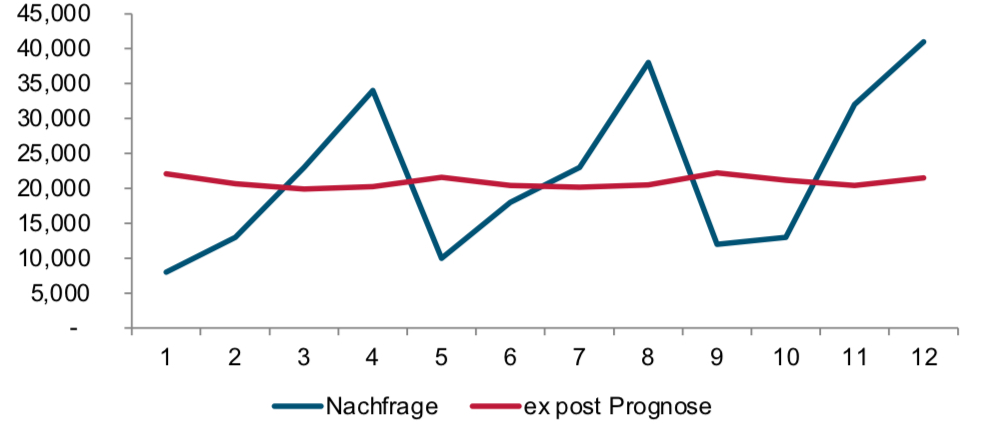
\includegraphics[width=0.5\linewidth]{UE11.jpg}\\[5cm]
\end{figure}

\item 2. Ordnung: trendförmig ansteigende Nachfrage\\
Niveau der Zeitreihe steigt \textbf{linear}\\

\begin{figure}[h!]
  \centering % 居中显示图片
  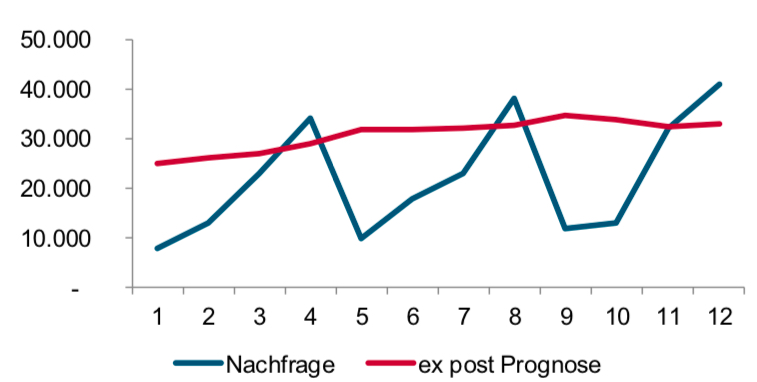
\includegraphics[width=0.5\linewidth]{UE12.jpg}
\end{figure}

\item 3. Ordnung: saisonal schwankende Nachfrage\\
Niveau der Zeitreihe steigt \textbf{linear}\\

\begin{figure}[h!]
  \centering % 居中显示图片
  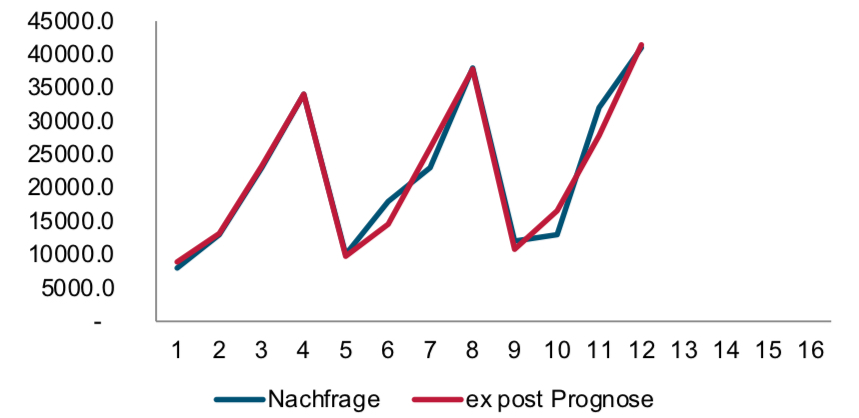
\includegraphics[width=0.5\linewidth]{UE13.jpg}
\end{figure}

\end{itemize}

%%%%%%%%%%%%%%%%%%%%
\newpage

\section{Beschaffungs- und Distributionslogistik}
\subsection{Beschaffungsstrategie}
\begin{itemize}
\item Klassifizierung der Beschaffungsartikel\\
\begin{figure}[h!]
  \centering % 居中显示图片
  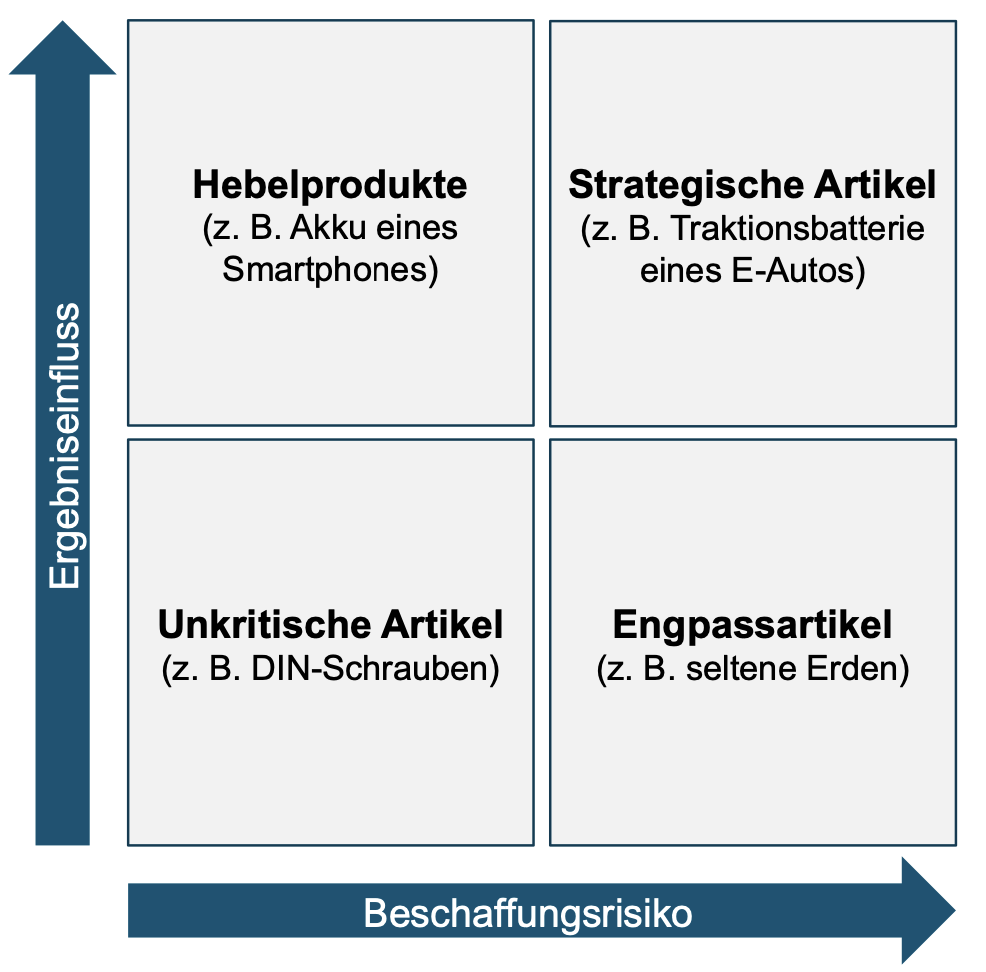
\includegraphics[width=0.6\linewidth]{VL31.png}\\
\end{figure}
\end{itemize}

\subsection{Beschaffungsstruktur}
\begin{itemize}
\item Global Sourcing vs. Regional Sourcing:\\
Nutzung weltweiter oder regionaler Beschaffungsstrukturen\\
\item Single vs. Multiple Sourcing\\
Nutzung eines oder mehrerer Lieferanten für die gleichen Teile\\
\item Modular vs. Unit Sourcing\\
Beziehung einer Baugruppe auf Bauteil- oder Baugruppenebene
\end{itemize}

\subsection{Bereitstellungskonzepte}
\begin{itemize}
\item Auftragsbezogene Beschaffung: (有了订单 再买货物)\\
\begin{figure}[h!]
  \centering % 居中显示图片
  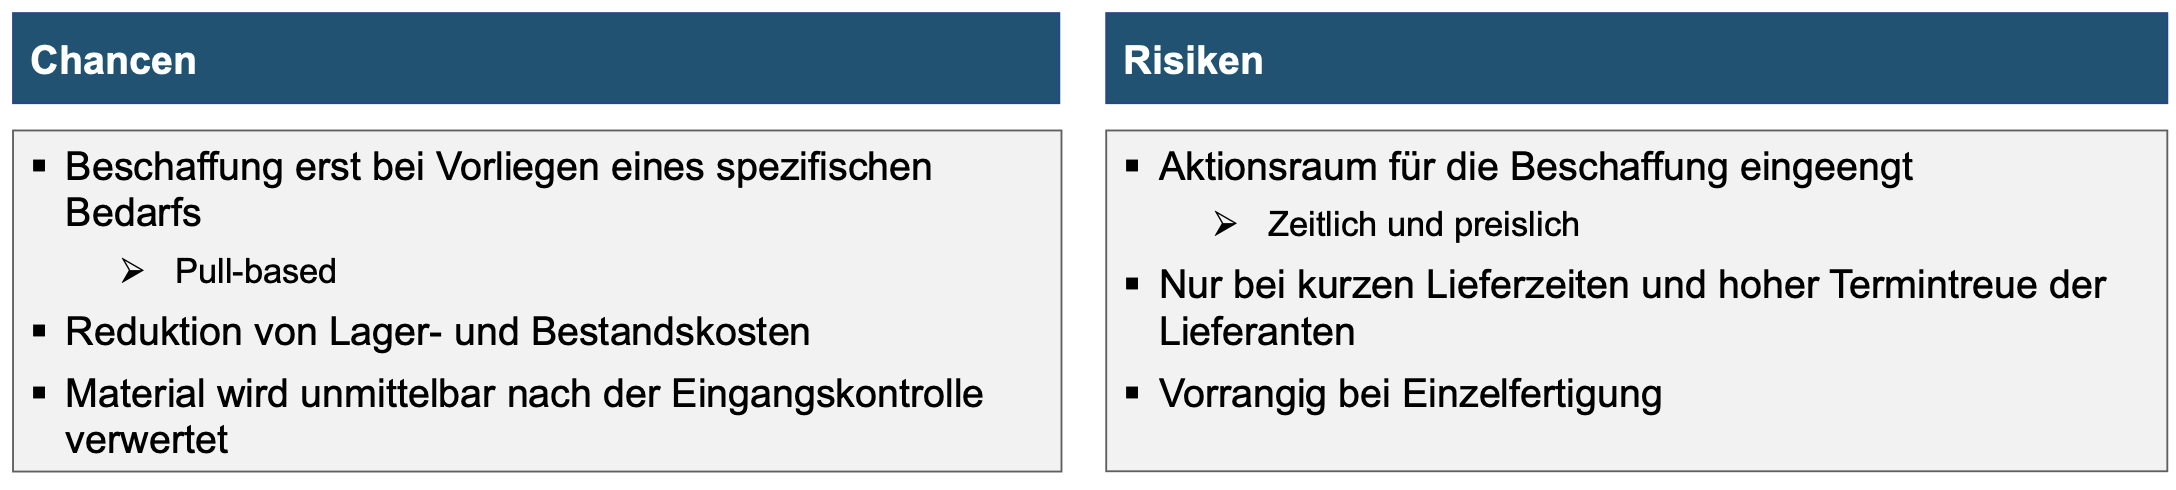
\includegraphics[width=0.7\linewidth]{VL32.png}\\
\end{figure}
Nachteil: \textcolor{red}{Hohe Unsicherheit}

\item Vorratsbeschaffung: (积累库存)\\
\begin{figure}[h!]
  \centering % 居中显示图片
  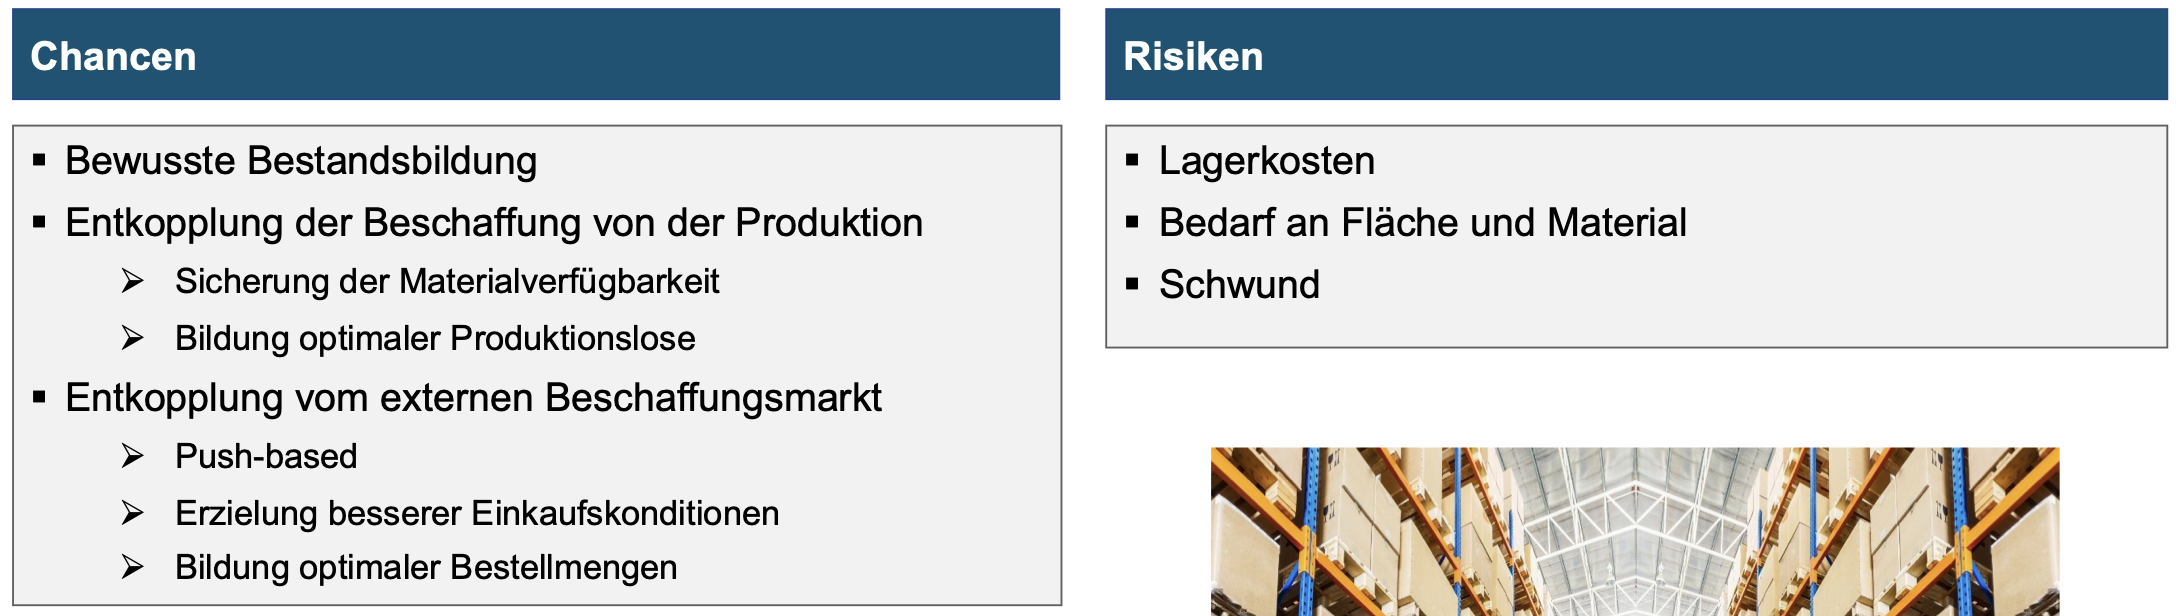
\includegraphics[width=0.7\linewidth]{VL33.png}\\
\end{figure}
Nachteil: \textcolor{red}{Hohe Lagerkosten}

\item Just In Time \& Just In Sequence\\
根据上述两个方法 引入的改良手段\\
Ziel: \textcolor{blue}{Möglichst nachfragegenaue Produktion und Beschaffung}


\item Produktionssynchrone Beschaffung: (边生产边买)\\
\begin{figure}[h!]
  \centering % 居中显示图片
  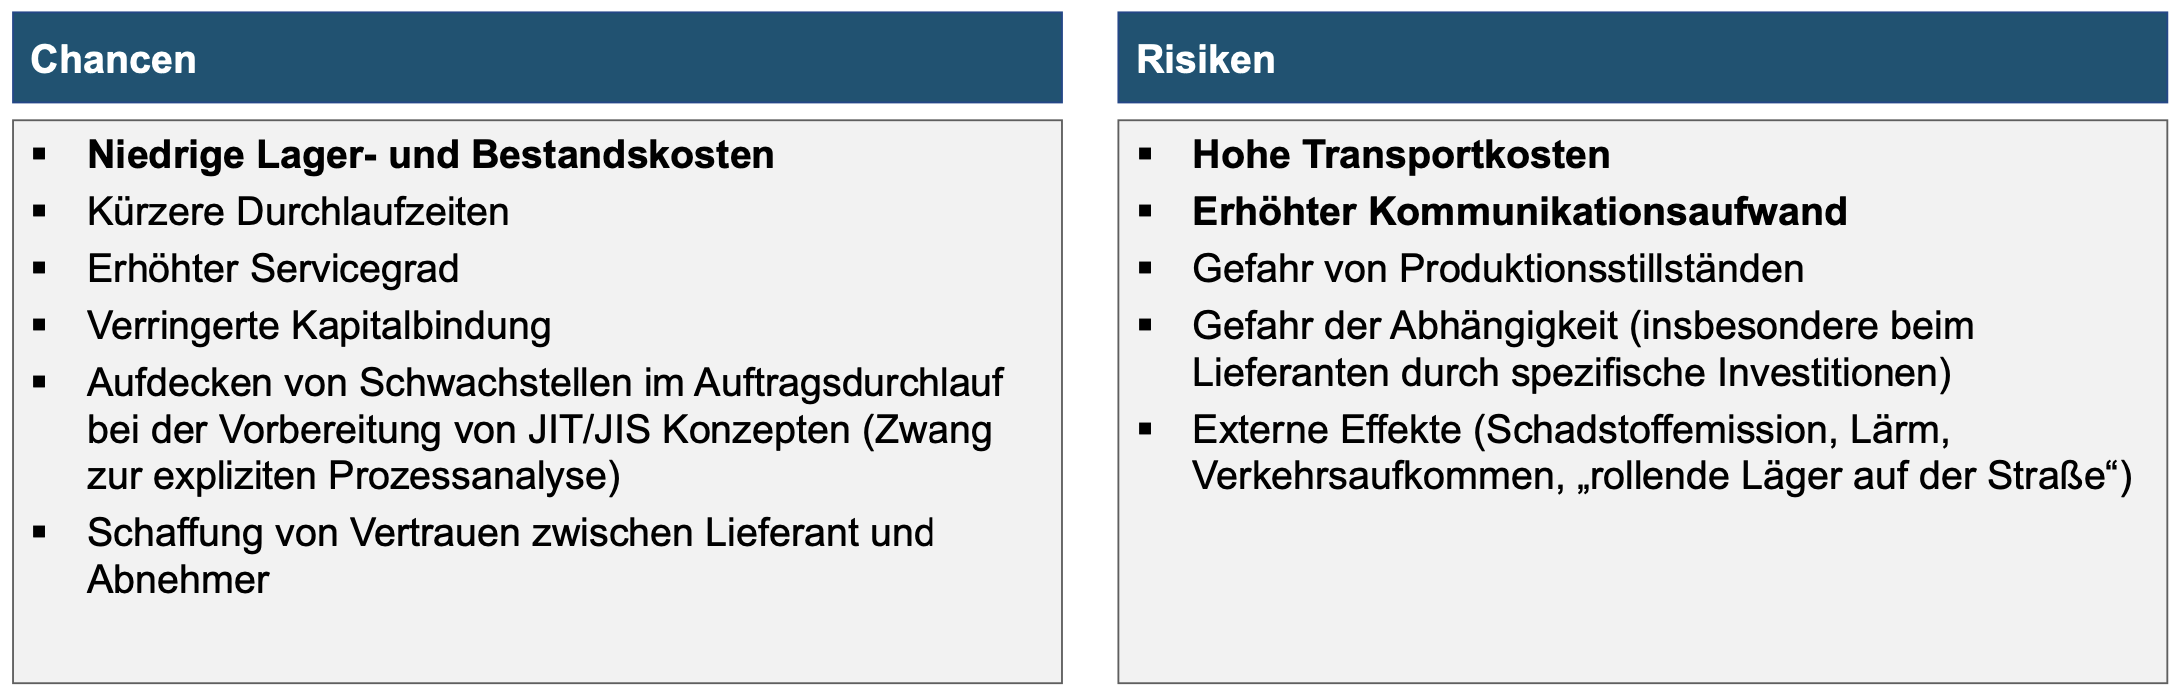
\includegraphics[width=0.7\linewidth]{VL34.png}\\
\end{figure}

\newpage
\item ABC-Analyse:\\
根据产品价值进行分类\\
\begin{figure}[h!]
  \centering % 居中显示图片
  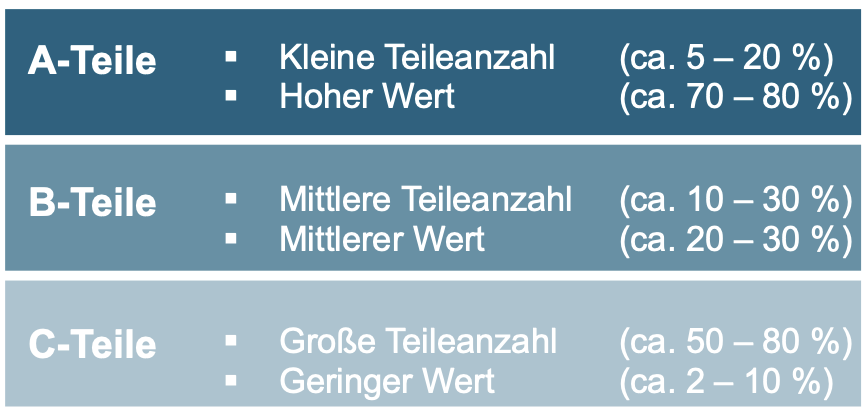
\includegraphics[width=0.4\linewidth]{VL35.png}\\
\end{figure}

\item XYZ-Analyse:\\
根据计划\&预测Sicherheit进行分类
\begin{figure}[h!]
  \centering % 居中显示图片
  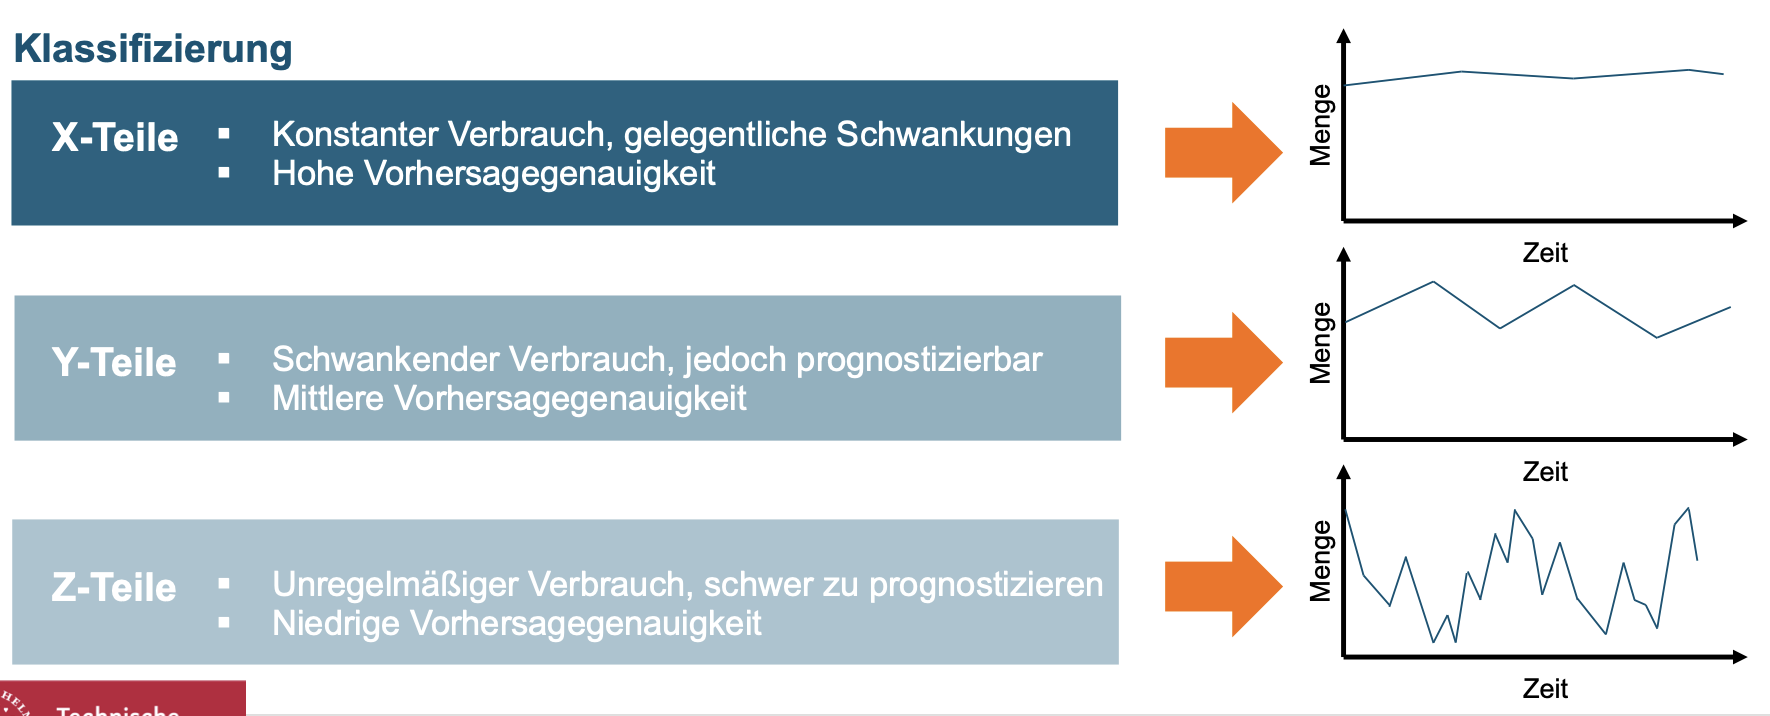
\includegraphics[width=0.6\linewidth]{VL36.png}\\
\end{figure}

\end{itemize}

\subsection{Distributionsstrategie}
\begin{itemize}
\item Werkslager 工厂仓库\\ 
nähe von Produktionsstätte

\item Zentrallager 中央仓库\\
Hoher Automatisierungsgrad und moderne Lagertechniken

\item Regionallager 区域仓库\\
Puffer zwischen Produktion und Absatzmarkt

\item Auslieferungslager 分发仓库\\
Dezentrale Ansiedlung im gesamten Verkaufsgebiet\\

\item vertikale \& horizontale Distributionsstruktur:\\[1mm]
vertikal: Lagerstufen 数量的定义\\[1mm]
horizontal: 不同Lagerstufen的仓库数量与位置的定义
\item zentrale vs dezentrale Lagerhaltung\\[1mm]
zentral: 产品组合广泛,运输时间长,贵重物品,一个供货商,少量大客户\\[1mm]
dezentral: 产品组合单一,运输快,产品便宜,多个供货商,许多小客户\\
\end{itemize}

\newpage
\section{Netzwerkplanung}
\subsection{Modelle zur Standortplanung}
Ziel: \textcolor{blue}{Transformation einer qualitativen Bewertung verschiedener sich ausschließender Handlungsalternativen in eine einheitliche quantitative Nutzenskala}\\[1mm]
将各种互斥行动方案的定性评估转化为统一的定量效益尺度

\subsection{Standortplanung in Netzen}
-Warehouse Location Probleme\\[1mm]
Ziel: \textcolor{blue}{Bestimmung eines oder mehrerer Standorte (und Transportmengen), so dass die Summe aus Fixkosten, variablen Betriebskosten und Transportkosten unter der Restriktion eines definierten Servicegrades minimiert wird}\\[1mm]
确定一个或多个位置(及运输量),以便在定义的服务等级的限制下,将固定成本、可变运营成本和运输成本的总和最小化

\newpage
\section{Produktionssegmentierung}
\subsection{Einführung}
Produktionssegment: Subsystem des Produktionsbereichs, welches eindeutig einem Organisationstyp zugeordnet
werden kann\\[1mm]
生产领域的子系统,可以明确地归属于一个组织类型。

\subsection{Assembly Line Balancing in der Fließproduktion}
根据产品数量 区分流水线种类
\begin{itemize}
\item Einprodukt-Fließproduktion (SALBP) 单品种物品流水线\\[1mm]
\textcolor{blue}{Produktion eines homogenen Produkts} mit hoher Qualität\\[1mm]
\textcolor{red}{Arbeitsinhalt konstant}

\item Mehrprodukt-Fließproduktion 多品种物品流水线\\[1mm]
\textcolor{blue}{Herstellung verschiedener Produkte} auf derselben Montagelinie

\item Multivarianten-Fließproduktion (MALBP) 多变量流水线\\[1mm]
\textcolor{blue}{Produktion verschiedener Varianten} auf derselben Montagelinie\\

\item 根据ZF区分SALBP \textbf{\textcolor{red}{Klausur Frage}}\\[1mm]
\begin{figure}[h!]
  \centering % 居中显示图片
  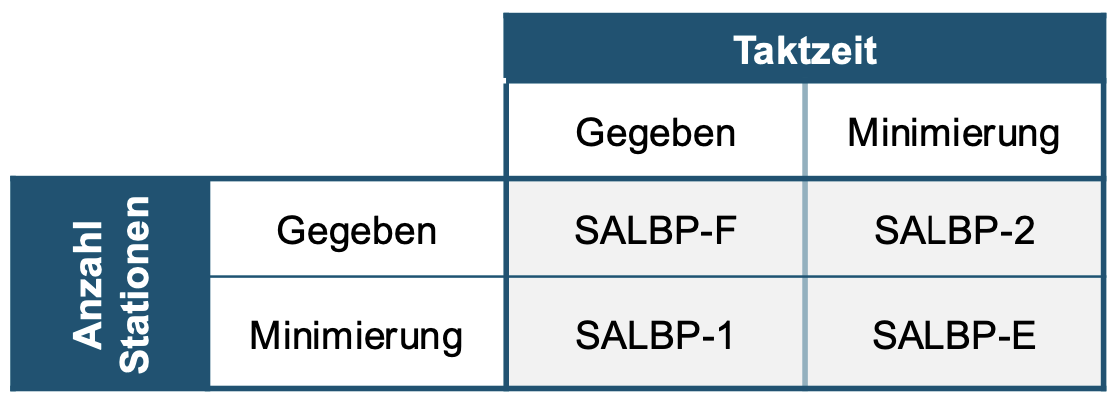
\includegraphics[width=0.4\linewidth]{VL51.png}
  \caption*{F:Machbarkeit, E:Effizient} % 为图片添加说明文字 *去掉Figure 1
\end{figure}
 
SALBP-1: Minimierung Anzahl, Taktzeit gegeben\\[1mm]
SALBP-2: Anzahl gegeben, Minimierung Taktzeit\\[1mm]
SALBP-F: beide gegeben \textcolor{blue}{所以牛逼}\\[1mm]
SALBP-E: beide Minimierung \textcolor{blue}{所以高效}

\end{itemize}


\newpage
\section{Produktionsprogrammplanung}
\subsection{Beschäftigungsglättung}
-aggregierte Gesamtplanung 整体聚合规划\\[1mm]
\begin{itemize}
\item Ausgleich von unterschiedlichen Kapazitätsbeanspruchungen der Produktionsstätten im Zeitablauf eines oder mehrerer
Jahre\\[1mm]
在一年或多年的时间跨度内,平衡生产设施不同的产能需求
\end{itemize}

\subsection{Kapazitierte Hauptproduktionsprogrammplanung}
-kurzfristige Produktionsprogrammplanung\\[1mm]
\begin{itemize}
\item Festlegung der konkreten Endproduktmengen in den einzelnen Perioden des unmittelbar bevorstehenden Planungszeitraums innerhalb einer Produktionsstätte\\[1mm]
在生产设施内,为即将到来的规划时期的每个阶段确定具体的最终产品数量
\end{itemize}


\newpage
\section{Bestandsmanagement}
Bestandsmanagement beschäftigt sich mit der Betrachtung aller im Unternehmen vorhandenen Lagerbestände mit dem Ziel, \textcolor{blue}{die Kapitalbindung zu senken und eine größere Kapitalumschlagshäufigkeit} im Unternehmen zu erzielen\\[1mm]
库存管理涉及对公司内所有现有库存的审视,目的是降低资本占用,并在公司内实现更高的资本周转率\\

\begin{figure}[h!]
  \centering % 居中显示图片
  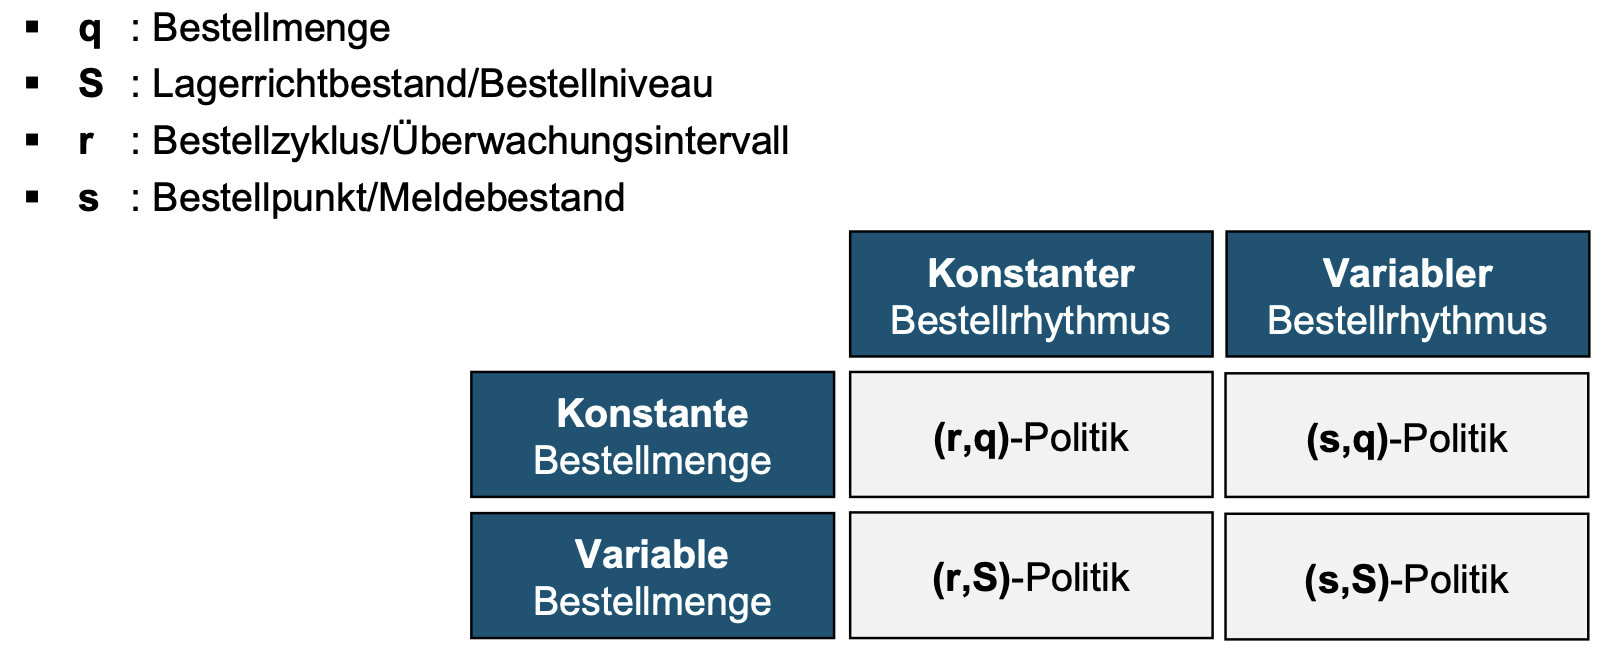
\includegraphics[width=0.8\linewidth]{VL71.png}
\end{figure}

\newpage
\section{Losgrößenplanung – Teil 1}
\begin{itemize}
\item Methoden der Losgrößenplanung:\\[1mm]
\textbf{sequenzielle Planung} - sukzessive Bestimmung von Bedarfen, Losgrößen und Terminen\\
顺序规划 - 逐步确定需求, 批量和时间表

\begin{enumerate}
\item programmorientierte Bedarfsermittlung
\item Losgrößenbestimmung
\end{enumerate}

\item Modell SLULSP - Verbalformulierung\\[1mm]
ZF: Summer der \textcolor{blue}{Kosten (Lager- und Rüstkosten) minimieren}\\[1mm]
\textcolor{red}{Problem}: Interdependenzen zwischen Mengen-, Termin- und Losgrößenplanung werden vernachlässigt

会导致: \textbf{Nicht realisierbare Pläne, Lieferterminschwierigkeiten}


\begin{figure}[h!]
  \centering % 居中显示图片
  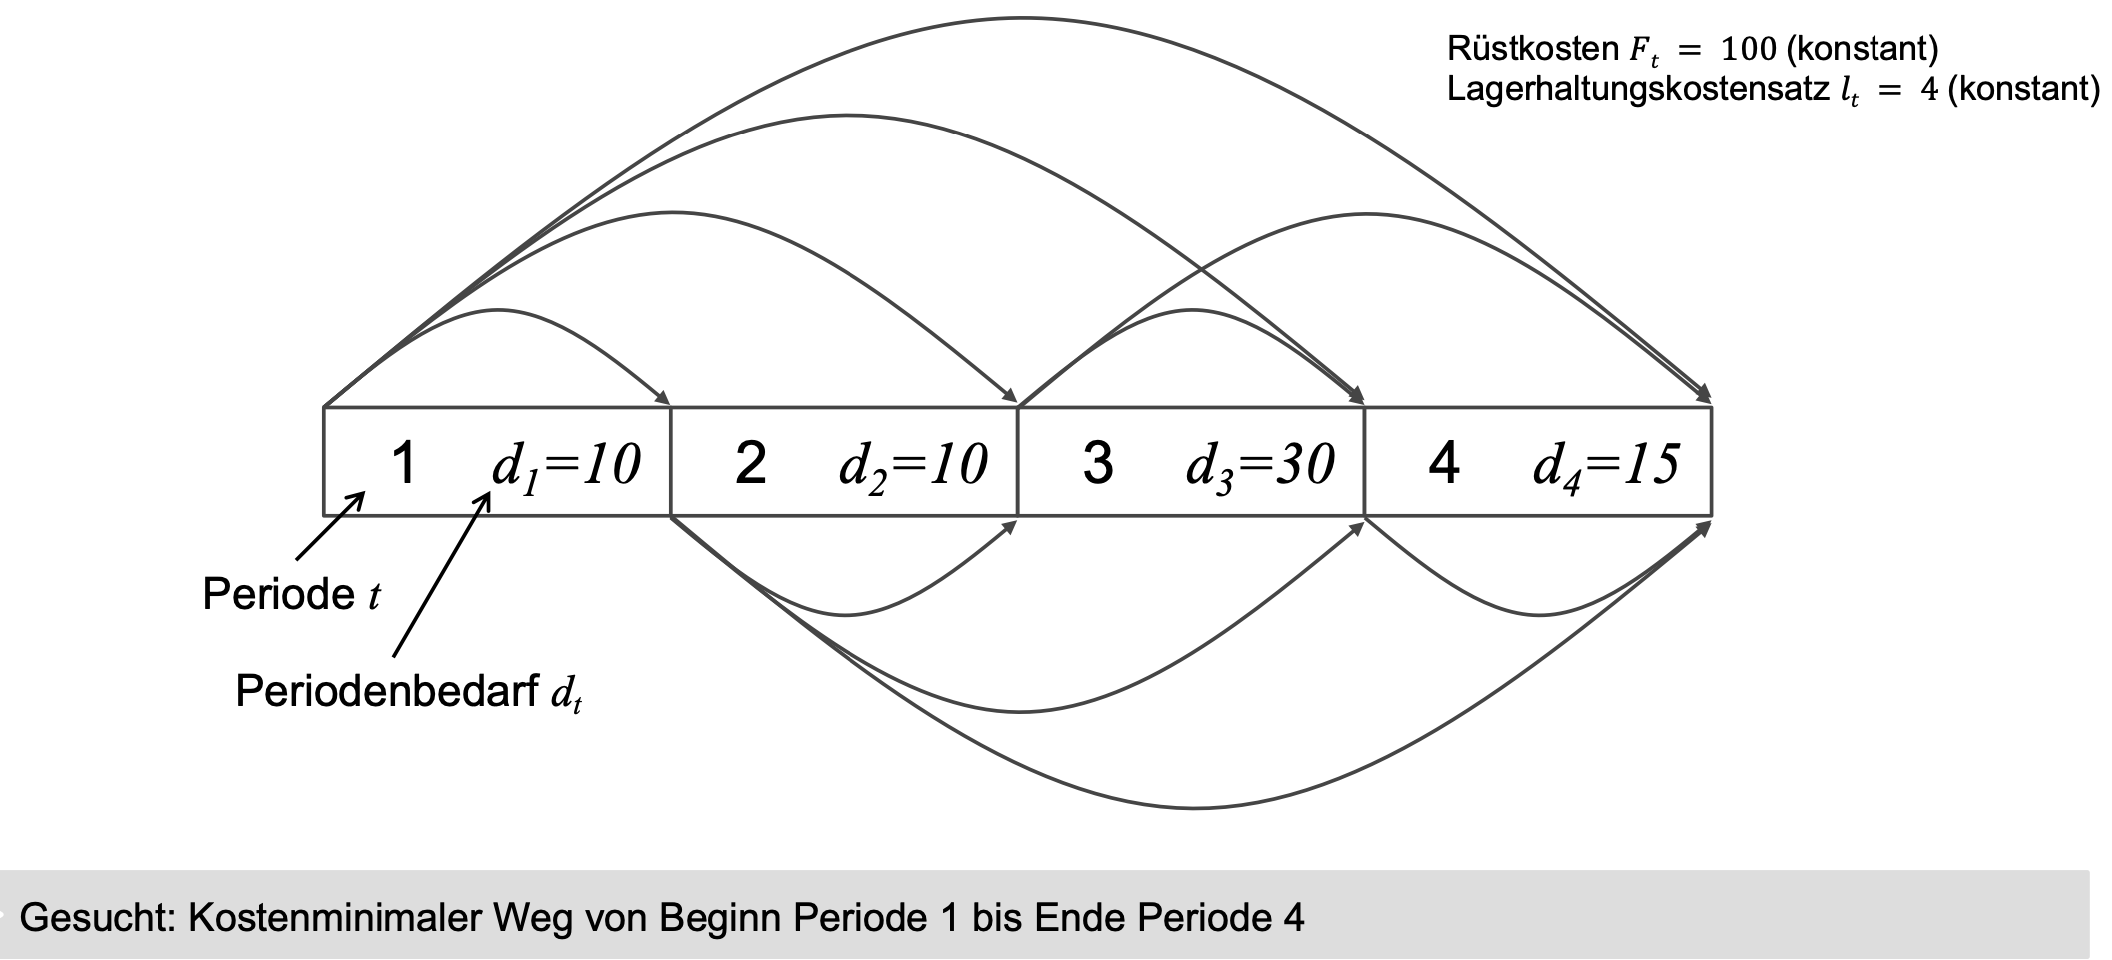
\includegraphics[width=0.9\linewidth]{VL81.png}
\end{figure}
\end{itemize}

\newpage
\section{Losgrößenplanung – Teil 2}
\begin{itemize}
\item Methoden der Losgrößenplanung:\\[1mm]
\textbf{simultane Planung} - Mehrstufige kapazitierte Losgrößenplanung\\
同时规划 - 多级容量约束的批量规划

\item Modell MLCLSP
ZF: Summer der \textcolor{blue}{Kosten (Lager- und Rüstkosten) minimieren}\\[1mm]
\textcolor{green}{Vorteil}: 顾及了Struktur- und zeitliche Zusammenhänge von Erzeugnissen

\item Fließproduktionslinie 流水线的优缺点\\[1mm]
V: sehr hohe Auslastung\\[1mm]
N: geringe Flexibilität

\end{itemize}



\end{CJK*}
\end{document}
